%!TEX root=thesis.tex
\section{Surface Theory}

  Investigating the properties of surfaces will form the basis on which our journey towards Minimal Surfaces rests. We will brave the perils that come in defining surfaces, and then use calculus on these surfaces to approximate the behavior at a point, then further extract information about the surface by extending on that approximation. Along the way we will uncover and derive various techniques used for analyzing these surfaces, some of which we will bring along with us to Minimal Surfaces, others are interesting nonetheless and help to illustrate some of the connections between Differential Geometry and various other branches of mathematics. In this chapter, we will also look at parallels between these surfaces in $\RR^3$ and higher dimensional Riemannian manifolds, though only briefly. In general our reference for this section will be~\cite{MP77} which, while not as recent as some other texts, gives a clean, if compact, view of the subject.

\subsection{Defining Surfaces in $\RR^3$}

  % Subsection introduction.
  Defining surfaces is not particularly difficult, but our methods require a set of considerations that can be subtle. We will first define a \emph{simple surface}, or coordinate patch, which represents a small open section of a larger surface. After considering that, we define a \emph{coordinate transformation}, a type of function whose presence between these patches implies geometry-preserving properties. That done, we finally build up surfaces using an open covering of these coordinate patches, with the requirement that a coordinate transformation exist on their intersection. Along the way, we will have plenty of examples to illustrate specific techniques and concepts introduced.

  \begin{unno_rem}
    Before proceeding we want to clarify the situation regarding notation. Differential geometry has had many influences over the years, and even a comparison of modern texts will show some divergence in notation used. As our time together is short and our desire to cause trouble small, we will lay out our conventions explicitly.

    We will be dealing with several varieties of functions, some more than others. For vector-valued functions from $\RR^2$ to $\RR^3$ we will almost always use a bold symbol (a notable exception being $f$, which does not look proper bold). Examples include $\bx$, $\by$, and $\bg$. We will always notate these functions parametrically, and indicate the individual coordinate functions using a normal-faced symbol matching the main function symbol and a superscript index. Example:
    \[
      \bx = \left(x^1, x^2, x^3\right).
    \]
    For the parameters, or inputs, to these functions, when appropriate we will use $u$ and $v$ to refer to the first and second parameter, respectively. As an example, observe
    \[
      \bx(u, v) = (x^1(u, v), x^2(u, v), x^3(u, v))
    \]
    Where more parameters are needed, or where the parameter used is dependent on some external value, we may take a single value (typically $u$ or $v$) and denote whether it is the first or second parameter with an upper index. To differentiate between parameters and coordinate functions, when both use upper indices, we can discern their meaning in a context by concentrating on the letters used. 

    There are several occassions where we will need derivatives. For single-parameter functions we will use prime notation (but reserve the right to use the prime to indicate a separate, but related space from another space, as in Definition~\ref{def:surface}). For functions with multiple parameters, we may take one of several paths, depending on which is most appropriate.

    We may use a numerical subscript on the bold-faced function symbol to indicate the partial derivative on the $i$-th parameter, as in 
    \[
      \bx_i = \frac{\del \bx}{\del u^i},
    \]
    and will usually do so where having the number itself helps us see how the different derivatives and tensors work together. This is also useful in situations where the parameter to use depends on a variable external to the expression in which it is contained.

    Where we are dealing with a single, isolated function that has been defined using $u$ and $v$ as parameters, we may denote the partial derivative on one or the other by setting it as a subscript on the symbol used for the function.
  \end{unno_rem}

  \begin{defn} % def: Simple Surface
    Let $\sU$ be an open subset of $\RR^2$, then a $C^k$ function $\bx: \sU \to \RR^3$, with $(k \ge 1)$ written $\bx(u^1, u^2)$, is known as a \emph{simple surface} if it is injective and regular. In order for $\bx$ to be \emph{regular},
    \[
      \frac{\partial\bx}{\partial u^1} \times \frac{\partial\bx}{\partial u^2} \neq \zero
    \]
    must be true across the domain of $\bx$.

    We may also refer to a simple surface as a \emph{patch} or \emph{coordinate patch}, the emphasis of which is that we build up surfaces as a patchwork of these simple surfaces, as we will see later.
  \end{defn}

  This definition may be unclear at first glance but we can break it down. A $C^k$ function is one that is differentiable at least $k$ times and whose $k$-th derivative is continuous. Then conceptually, the regularity of $\bx$ ensures that the mapping of $\sU$ to $\RR^3$ does not create any sharp creases or corners and, perhaps more technically relevant to our purposes, it also implies that the partial derivatives form a linearly independent set. This will be critical later on.

  \begin{ex} % ex: Monge Patch example
    \label{ex:monge}
    Before going any further we introduce the \emph{monge patch}, a simple surface that we will revisit periodically as a simple example on which we can carry out our calculations. Let $f(x, y) = z$ be a function, then we can parameterize a patch as follows: $\bx(u, v) = (u, v, f(u, v))$. Notice that
    \begin{equation*}
      \frac{\partial\bx}{\partial u} \times \frac{\partial\bx}{\partial v} = \left(-\frac{\partial f}{\partial u}, -\frac{\partial f}{\partial v}, 1\right) \neq \zero,
    \end{equation*}
    thus it is a simple surface.
  \end{ex}

  In the example below, we make use of the notation
  \[
    \bx_i = \frac{\del\bx}{\del u^i},
  \]
  which we have discussed previously.

  \begin{ex} % ex: Surface of revolution
    \label{ex:revolution}
    Another example is that of the generic \emph{surface of revolution}. Let $\bg:\RR\to\RR^2$ be given by $\bg(t) = (r(t), z(t))$ with $r(t) > 0$. The surface of revolution generated by this curve (via rotation about the $z$-axis), is given by
    \[
      \bx(t, \theta) = (r(t)\cos\theta, r(t)\sin\theta, z(t)) \ .
    \]

    % NOTE: p15
    Assuming the curve is regular and injective, we can show that a surface of revolution is a simple surface by checking its properties against the requirements of the definition. (A curve, say $\ba : (a, b) \to \RR^3$ is considered \emph{regular} when $\frac{d\ba}{dt} \neq \zero$ for any $t$ in $(a, b)$.)

    A quick calculation yields the following:
    \begin{align*}
      \bx_1 &= (r^\prime(t)\cos{\theta}, r^\prime(t)\sin{\theta}, z^\prime(t))\\
      \bx_2 &= (-r(t)\sin{\theta}, r(t)\cos{\theta}, 0)\\
      \bx_1 \times \bx_2 &= (-z^\prime(t) r(t) \cos{\theta}, -z^\prime(t) r(t) \sin{\theta}, r^\prime(t)r(t)).
    \end{align*}
    Then since the original curve was regular, $r^\prime(t) \neq 0$ and $z^\prime(t) \neq 0$. This combined with our assumption that $r(t) > 0$ implies that at no point is $\bx_1 \times \bx_2 = \zero$. Hence a surface of revolution is a simple surface.
  \end{ex}

  % PTODO: Example of an irregular surface

  \begin{defn} % def: Coordinate transformation definition (LOC: p79)
    Let $\sU, \sV$ be open subsets of $\RR^2$. A $C^k$ \emph{coordinate transformation} is a bijective $C^k$ function $f: \sV \to \sU$ whose inverse $g:\sU \to \sV$ is also of class $C^k$. (Essentially we're defining a $C^k$-diffeomorphism between $\sU$ and $\sV$.)
  \end{defn}

  As we continue we will lean heavily on the structure-preserving properties of these coordinate transformations, so we will take some time with them now to fully appreciate their impact. Let $f(v^1, v^2)$ be a function from $\RR^2$ to itself and recall the \emph{Jacobian} of $f$ is the matrix-valued function of partial derivatives, denoted $J(f)$ given by
  \begingroup
    \renewcommand*{\arraystretch}{1.4}
    \begin{align*}
      J(f) &= \left(
      \begin{array}{cc}
        \frac{\del f^1}{\del v^1} & \frac{\del f^1}{\del v^2}\\
        \frac{\del f^2}{\del v^1} & \frac{\del f^2}{\del v^2}
      \end{array}
      \right),
    \end{align*}
    where each $f^i$ is the $i$-th coordinate function for $f$
  \endgroup

  \begin{lem}
    If $f:\sV \to \sU$ be a coordinate transformation, then $J(f)$ is nonsingular.
  \end{lem}

  \begin{proof}
    We can write $f(v^1, v^2) = (f^1(v^1, v^2), f^2(v^1, v^2))$. Then since $f$ is a coordinate transformation there exists an inverse function $g$, which we will denote $g(u^1, u^2) = (g^1(u^1, u^2), g^2(u^1, u^2))$. Then since $f$ and $g$ are inverses we have
    \begin{align*}
      f^1(g^1, g^2) &= u^1\\
      f^2(g^1, g^2) &= u^2 \ .
    \end{align*}
    Taking the partial derivative of each on $u^1$ and $u^2$ yields
    \newcommand{\fdg}[3]{\frac{\del f^{#1}}{\del v^{#2}} \cdot \frac{\del g^{#2}}{\del u^{#3}}}
    \begin{equation*}
      \begin{aligned}[c]
        \fdg{1}{1}{1} + \fdg{1}{2}{1} &= 1\\
        \fdg{2}{1}{1} + \fdg{1}{2}{1} &= 0
      \end{aligned}\qquad
      \begin{aligned}[c]
        \fdg{1}{1}{2} + \fdg{1}{2}{2} &= 0\\
        \fdg{2}{1}{2} + \fdg{2}{2}{2} &= 1 \ ,
      \end{aligned}
    \end{equation*}
    which is certainly nonsingular. Then since $f$ was generic, coordinate transformations have nonsingular Jacobian.
  \end{proof}

  % TODO: Finish the proof below
  \begin{lem}
    % TODO: Fix wording.
    Let $\bx: \sU \to \RR^3$ be a simple surface and $f:\sV \to \sU$ a coordinate transformation. The function $\by$ defined as $\by = \bx \circ f: \sV \to \RR^3$ is a simple surface with the same image as $\bx$.
  \end{lem}
  \newcommand{\xdf}[2]{\frac{\del\bx}{\del u^{#1}}\cdot\frac{\del f^{#1}}{\del v^{#2}}}
  \newcommand{\df}[2]{\frac{\del f^{#1}}{\del v^{#2}}}
  \newcommand{\dx}[1]{\frac{\del\bx}{\del u^{#1}}}
  \begin{proof}
    Since both $\bx$ and $f$ are injective, so too is $\by$. Then we have
    \begin{align*}
      \by(\sV) &= \bx(\sU)
    \end{align*}
    by the properties stated above. The chain rule shows us that
    \begin{equation*}
      \by_\alpha = \bx_1f^1_\alpha + \bx_2f^2_\alpha = \sum \bx_if^i_\alpha,
    \end{equation*}
    (using $f^i$ to denote the specific parameter function for $\bx$ and the $\alpha$ subscript to denote the partial derivative of $f^i$ on $\alpha$). We compute
    \begin{align*}
      \left(\xdf{1}{1} \right.&\left.+ \xdf{2}{1}\right) \times \left(\xdf{1}{2} + \xdf{2}{2}\right)\\
      &= \left(\left(\xdf{1}{1} + \xdf{2}{1}\right) \times \xdf{1}{2}\right) + \left(\left(\xdf{1}{1} + \xdf{2}{1}\right) \times \xdf{2}{2}\right)\\
      &=\left(\xdf{1}{1} \times \xdf{1}{2}\right) + \left(\xdf{2}{1} \times \xdf{1}{2}\right) + \\
      &\quad\quad\quad\quad\quad\quad\quad\quad\quad\quad\quad\quad\quad\quad\quad\left(\xdf{1}{1} \times \xdf{2}{2}\right) + \left(\xdf{2}{1} \times \xdf{2}{2}\right)\\
      &=0 + \left(\xdf{2}{1} \times \xdf{1}{2}\right) + \left(\xdf{1}{1} \times \xdf{2}{2}\right) + 0\\
      &=\df{2}{1}\cdot\df{1}{2}\left(\dx{2} \times \dx{1}\right) + \df{1}{1}\cdot\df{2}{2}\left(\dx{1} \times \dx{2}\right)\\
      &=\df{2}{1}\cdot\df{1}{2}\left(-\dx{1} \times \dx{2}\right) + \df{1}{1}\cdot\df{2}{2}\left(\dx{1} \times \dx{2}\right)\\
      &=\left(\df{1}{1}\cdot\df{2}{2} - \df{2}{1}\cdot\df{1}{2}\right)\left(\dx{1} \times \dx{2}\right)\\
      &=\text{det}(J(f))\left(\dx{1} \times \dx{2}\right)
    \end{align*}
    then since $J(f)$ is nonzero we have that $\by$ is regular and hence a simple surface.
  \end{proof}

  Before defining surfaces, we need to put an additional restriction on the coordinate patches that we build them with.

  Consider the inverse function for a coordinate patch $\bx$ from some subset $M$ of $\RR^3$ back to $\sU$, $\bx^{-1}: M \to \RR^2$. We will say that this function is \emph{continuous} at a point $p$ if there is a neighborhood $U_p$ around the point such that $\bx^{-1}(U_P)\subset \sU$. The patch $\bx$ is considered \emph{proper} if $\bx^{-1}$ is continuous for all $P \in \bx(\sU)$. Notice that this is a property of the inverse function, not the function defining the simple surface itself. Continuity of $\bx$ is implied because it is a $C^k$ function.

  \begin{defn} % def: Surface (LOC: p89)
    \label{def:surface}
    A $C^k$ \emph{surface} in $\RR^3$ is a subset $M \subset \RR^3$ such that for every point $p \in M$ there is a proper $C^k$ coordinate patch whose image is in $M$ and which contains an $\eps$-neighborhood of $p$ for some $\eps > 0$. Furthermore, if both $\bx: \sU \to \RR^3$ and $\by: \sV \to \RR^3$ are such coordinate patches with $\sU^\prime = \bx(\sU), \sV^\prime = \by(\sV)$, then $y^{-1} \circ \bx: (x^{-1}(\sU^\prime \cap \sV^\prime)) \to (y^{-1}(\sU^\prime \cap \sV^\prime))$ is a $C^k$ coordinate transformation.
  \end{defn}

  We can see a demonstration of the above definition in Figure~\ref{fig:transformation}

  In many cases we will only consider a single patch, but this helps us to see the context of our discussion. Similarly, in most cases we work with smooth functions, but thus far only make the requirement of being $C^k$ differentiable. We will take it as a given that the surfaces we are working with are path connected, so there's no trouble in finding an arbitrary curve between any points on them (this helps avoid trivial cases and/or conditions on some of the proofs to follow). 

  As stated previously, coordinate transformations have a preserving property but that isn't the whole story. It is really the case that we define a property \emph{as} geometric when we can show that it is preserved under coordinate transformation. This will ensure that the property exists for a surface regardless of parameterization which is important here since it is very likely that multiple such parameterizations exist.

  % TODO: Label U and V.
  % TODO: Change arrows.
  % TODO: Surface surrounding mapped regions.
  % TODO: \bx
  \begin{figure}[b] % fig: Coordinate transformation
    \centering
    \begin{tikzpicture}
      [region/.style={ellipse,draw,x radius=20pt,y radius=10pt,inner sep=0pt,minimum height=6mm,minimum width=12mm}]
      % Bottom left ellipse.
      \node (U) at (3,2) [
        region,
        rotate=8,
        pattern=right crosshatch,
        path picture={
          \pgftransformreset
          \node (UV) [region,rotate=10,above right=-0.3cm and 0.1cm of U,pattern=left crosshatch] {};
        }
      ] {};
      
      \draw (1.5,1) -- (5,1);
      \draw (2,0.5) -- (2,3.5);

      % Bottom right ellipse.
      \node (V) at (9,2) [
        region,
        rotate=-25,
        pattern=left crosshatch,
        path picture={
          \pgftransformreset
          \node (VU) [region,rotate=10,above left=-0.3cm and 0.1cm of V,pattern=right crosshatch] {};
        }
      ] {};
      \draw (7.5,1) -- (11,1);
      \draw (8,0.5) -- (8,3.5);
      \draw [->] (U.east) to [bend left=15] node[auto,swap] {$y^{-1}\circ x$} (V.west);
      
      \node (U2) at (5,5) [region,rotate=10,pattern=right crosshatch] {};
      \node (V2) [region,rotate=10,above right=-0.3cm and 0.1cm of U2,pattern=left crosshatch] {};

      \draw [->] (U.north) to [bend left=15] node[auto] {$x$} (U2.west);
      \draw [->] (V.north) to [bend right=25] node[auto] {$y$} (V2.east);
    \end{tikzpicture}
    \caption{Coordinate Transformation}
    \label{fig:transformation}
  \end{figure}

  % TODO: Finish example of definition of the coordinate patches for a torus.
  One surface of revolution, the torus, has a patch given by the parameterization
  \[
    \bx(u, v) = ((2 + \cos u)\cos v, (2 + \cos u) \sin v, \sin u)
  \]
  with the domain $\sU = \buildset{(u, v) \in \RR^2}{-\pi < u, v < \pi}$.

  If we look at Figure~\ref{fig:torus} below we can see the areas not covered by this coordinate patch highlighted.
  \begin{figure}[t] % fig: Torus
    \centering
    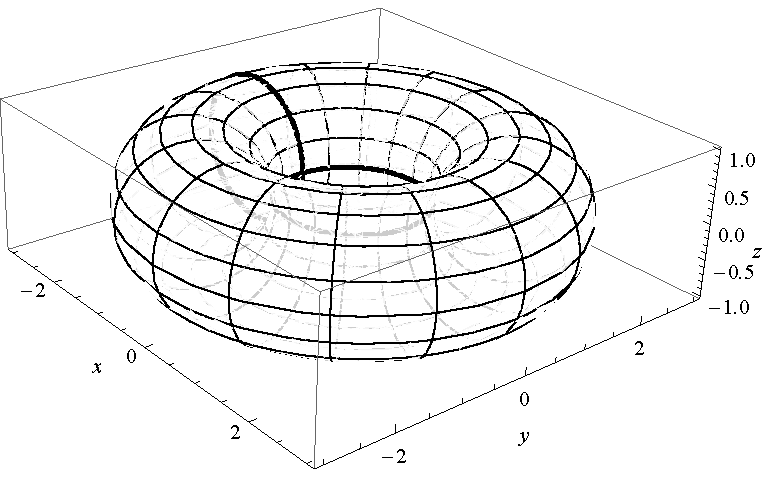
\includegraphics[width=0.5\textwidth]{figures/torus.pdf}
    \caption{Torus with single surface patch.}
    \label{fig:torus}
  \end{figure}
  In this case finding additional patches so the surface is covered is not difficult. We can use the same parameterization but with different bounds on the domain. If we let
  \begin{align*}
    \sU_1 &= \buildset{(u, v) \in \RR^2}{-\pi < u < \pi, \frac{3\pi}{4} < v < \frac{5\pi}{4}}\\
    \sU_2 &= \buildset{(u, v) \in \RR^2}{\frac{5\pi}{6} < u < \frac{7\pi}{6}, \frac{\pi}{4} < v < \frac{7\pi}{4}}\\
    \sU_3 &= \buildset{(u, v) \in \RR^2}{\frac{5\pi}{6} < u < \frac{7\pi}{6}, -\frac{3\pi}{4} < v < \frac{3\pi}{4}}
  \end{align*}
  with the same parameterization for each, these will cover the outside of the torus on the negative $x$ side, the inside of the torus on the negative $x$ side, and the inside of the torus on the positive $x$ side, respectively.

  % TODO: Check one of the intersections as a coordinate transformation

%%%%%%%%%%%%%%%%%%%%%%%%%%
%% Calculus On Surfaces %%
%%%%%%%%%%%%%%%%%%%%%%%%%%

\subsection{Calculus on Surfaces}

  In this portion of our exploration we will define a structure, the \emph{tangent plane}, on the surfaces introduced above. We will also show that tangent planes remain preserved under reparameterization, when considered on a surface meeting the coordinate transformation requirement we have imposed. The tangent plane will give us a linear approximation of the behavior of the surface at a specific point on which we will build our tools in the next section, and the fact that it is preserved under coordinate transformation will obviate the need to check each tensor individually.

  We consider two specific tangent vectors on a surface, corresponding to the derivative of the $x^1$ and $x^2$-parameter curves (the result of holding one parameter of a surface constant and varying the other). This is exactly the first and second parameter partial derivatives we've been using, $\bx_1$ and $\bx_2$.

  \begin{unno_rem}
    We typically consider the partial derivative as the tangent vector of a curve holding one parameter of the function constant, so planting the base of the vector at the point at which it is evaluated.
  \end{unno_rem}

  \begin{defn}
    The \emph{tangent plane} to a simple surface  $\bx: \sU \to \RR^3$ at the point $p = \bx(a, b)$ is the plane through $p$ perpendicular to $\bx_1(a, b) \times \bx_2(a, b)$. The \emph{unit normal} to the surface at $p$ is $\bn(a, b) = \frac{\bx_1 \times \bx_2}{\norm{\bx_1 \times \bx_2}}$, where the right-hand side is evaluated at $(a, b)$. Note that $\bn(a, b)$ exists because $\bx_1 \times \bx_2 \neq \zero$.
  \end{defn}

  \begin{unno_rem}
    There are a few things to notice here. First, as $\bx_1$ and $\bx_2$ form a basis for the tangent plane and the unit normal is perpendicular to both, all together these three vectors form a basis for $\RR^3$. This will be useful later on as we consider the second derivative of curves at a point and will calculate them to put it into the context of the tangent plane.
  \end{unno_rem}

  % Tangent plane preserved under coordinate transformation.
  \begin{prop}
    Let $\bx$ be a simple surface and $f:\sU\to\sV$ a coordinate transformation. Then, given $\by = \bx \circ f$, the tangent plane at a point on $\by$ is the same as that on the same point of $\bx$ and the normal is the same, up to sign.
  \end{prop}

  We can see the above by simply referencing our previous treatment of coordinate transformations.

  The condition on the sign of the unit normal is due to parameterizations of surfaces that are \emph{non-orientable} (e.g. Möbius strip). To ease our progress, we will take surfaces in examples and theorems to be orientable unless stated otherwise.

\subsection{Tensors and Operators on Surfaces}

  In this section we discover some of the tools that we will use to figure out the properties of surfaces in the next. Notice as we travel that the majority of these forms and tensors are really capturing very simple information, but we turn around and use them in combination to represent more complex or subtle properties of the surface. For this section assume that our operations are taking place on a simple surface and, as the tangent plane being \emph{geometric} (i.e. independent of parameterization) was shown in the last section, take these objects built upon it to inherit the same property.

  % First fundamental form and metric tensor
  \begin{unno_rem}
    One of the most fundamental operations in Euclidean space, allowing us notions of distance and angles between vectors, is the dot product (or more generally, the \emph{inner product}). We wish to have the same capability on our surface. To motivate our construction, consider a surface $M \subset \RR^3$, $P$ a point on the surface, and two vectors $\bX$ and $\bY$ tangent to $M$ at $P$. Since $\bx_1$, $\bx_2$ form a basis for the tangent plane, in which $\bX$ and $\bY$ lie, we can write them as a linear combination and further, compute their inner product (denoted henceforth as $\la\phantom{x},\phantom{x}\ra$) as follows:
    \begin{align*}
      \bX &= \sum X^i\bx_i\\
      \bY &= \sum Y^j\bx_j\\
      \la\bX, \bY\ra &= \sum X^iY^j\la\bx_i, \bx_j\ra \ .
    \end{align*}
    With this in mind we make the following definition.
  \end{unno_rem}

  \begin{defn}
    The \emph{metric coefficients}, or \emph{metric tensors} of a surface parameterized by coordinate patch $\bx$ are the functions defined by
    \[
      g_{ij}(u, v) = \la\bx_i(u, v), \bx_j(u, v)\ra \text{ or } g_{ij} = \la\bx_i, \bx_j\ra.
    \]

    Taking the metric coefficients as a single entity we have a matrix-valued function we can write as
    \[
      g_{ij} = \left(\begin{array}{cc}
        \la\bx_1, \bx_1\ra & \la\bx_1, \bx_2\ra\\
        \la\bx_2, \bx_1\ra & \la\bx_2, \bx_2\ra
      \end{array}\right).
    \]
    We can see that as the inner product is commutative, $g_{ij}$ is symmetric across $\bx$ (i.e. $g_{12} = g_{21}$). While it is important to note that the metric tensors are certainly dependent on the choice of coordinate patch, we will not take such issues upon ourselves, and refer to~\cite{MP77} for the resolution of those (page 97 has a listing of the various formulae relating the metric tensors and how they change under a choice of different coodinate patch).
  \end{defn}
  \begin{lem}
    \label{lem:gkl}
    Given $\bx$ a coordinate patch on some surface, let $g$ denote $\det(g_{ij})$ and $g^{kl}$ denote the $(k, l)$ entry of the inverse matrix to $g_{ij}$. Observe
    \begin{align*}
      g^{11} &= \frac{g_{22}}{g}\\
      g^{12} &= g^{21} = -\frac{g_{12}}{g}\\
      g^{22} &= \frac{g_{11}}{g}.
    \end{align*}
  \end{lem}

  \begin{ex}
    Using our definition above, let's find the metric coefficients for a surface of revolution. Recall the parameterization and first partial derivatives found in example~\ref{ex:revolution},
    \begin{align*}
      \bx_1 &= (r^\prime(t)\cos{\theta}, r^\prime(t)\sin{\theta}, z^\prime(t))\\
      \bx_2 &= (-r(t)\sin{\theta}, r(t)\cos{\theta}, 0) \ .
    \end{align*}
    Then calculating the relevant inner products yields
    \[
      g_{ij} = \left(\begin{array}{cc}
        \left(r^\prime(t)\right)^2 + \left(z^\prime(t)\right)^2 & 0\\
        0 & \left(r^\prime\right)^2
      \end{array}\right).
    \]
  \end{ex}

  % Second fundamental form
  \begin{unno_rem}
    When taking the second derivative on a coordinate patch we will denote it in much the same way as the first derivative
    \[
      \bx_{ij} = \frac{\partial^2\bx}{\partial u^j \partial u^i}.
    \]
  \end{unno_rem}

  % Coefficients of the second fundamental form
  \begin{defn}
    Let $\bx$ be a simple surface. We define the \emph{coefficients of the second fundamental form} as the functions $L_{ij}$, computed as $L_{ij} = \la\bx_{ij}, \bn\ra$. 
  \end{defn}

  % Christoffel Symbols
  \begin{defn}
    Let $\bx$ be a simple surface. The \emph{Christoffel symbols} are the functions $\Cfl$, with $1 \le i, j, k \le 2$ defined as
    \[
      \Cfl = \la\bx_{ij}, \bx_{1}\ra g^{1k} + \la\bx_{ij}, \bx_{2}\ra g^{2k},
    \]
    where $g^{lk}$ is an entry in the inverse matrix to $g_{ij}$ defined as in Lemma~\ref{lem:gkl}. 
  \end{defn}
  
  We will use the coefficients of the second fundamental form and the Christoffel symbols to measure the normal component and tangential (i.e. in the direction of $\bx_1$ and $\bx_2$) component of vectors, respectively.
  
  In each of these cases we note that both tensors are defined extrinsically. In the case of the coefficients of the second fundamental form this can not be helped (as it is inextricably linked to $\bn$, which is certainly extrinsic). For the Christoffel symbols however we do have an intrinsic formula which we state here.

  \begin{unno_rem}
    In general when juggling intrinsic/extrinsic, a good rule of thumb is that if it is based solely on the metric tensor, or something else which can be shown in terms of the metric tensor alone, it's intrinsic!
  \end{unno_rem}

  \begin{prop}[Proposition 4.3 of~\cite{MP77}]
    Let $\bx$ be a coordinate patch and $g_{ij}$ its metric coefficients. Then we can define the Christoffel symbols intrinsically as
    
    \begin{equation}
      \label{eq:intrinsic_cfl}
      \cfl{i}{j}{l} = \frac{1}{2} \sum_{k = 1}^2 g^{kl} \left(\frac{\del g_{ik}}{\del u^j} - \frac{\del g_{ij}}{\del u^k} + 
    \frac{\del g_{kj}}{\del u^i}\right).
    \end{equation}
  \end{prop}

  % PTODO: Computation of Christoffel symbols
  %\begin{ex}
  %  Example of computing Christoffel symbols
  %\end{ex}
  
  With these we can make the following proposition.

  \begin{prop}[Proposition 4.2 of~\cite{MP77}]
    Let $\bx: \sU \to \RR^3$ be a simple surface. Then
    \begin{enumerate}
      \item[(a)] (Gauss's formulas)
      \begin{equation*}
        \bx_{ij} = L_{ij}\bn + \sum_k\Cfl\bx_k
      \end{equation*}
      \item[(b)] for any unit speed curve, $\bg(s) = \bx(\gamma^1(s), \gamma^2(s))$
      \begin{equation*}
        \bk_n = \sum_{i, j} L_{ij}\left(\gamma^i\right)^\prime \left(\gamma^j\right)^\prime
      \end{equation*}
      and
      \begin{equation*}
        \label{eq:gdsc_intrinsic}
        \bk_g\bS = \sum_k\left[\left(\gamma^k\right)^{\prime\prime} + \sum_{i, j}\Cfl\left(\gamma^i\right)^\prime \left(\gamma^j\right)^\prime\right]\bx_k,
      \end{equation*}
      where $\bS = \bn \times \bT$ is the intrinsic normal of $\bg$ and $\bk_n$ and $\bk_g$ are defined as in Definition~\ref{def:curvature}.
    \end{enumerate}
  \end{prop}

  We mentioned this earlier, as each of $\bx_1, \bx_2, \bn$ are orthogonal, we can use them to form a basis for $\RR^3$, and we show here the relationship between the tensors introduced and the second derivative. The definitions make sense because $\bn$ is the unit normal and the inner product suffices to give the coefficient, and while the Christoffel symbols are a little more complicated in comparison this is just the result of using the unit normal as sort of the `basis', the place to start when determining the coefficients.

  The second and third equations we note here for context but will not reference until dealing with curvature in the next section.

  Our goal with the next operator is to get an impression of the change in the normal to the surface and use this to make determinations about how the surface is curving in space. We make the following definition to that end.

  \begin{defn}
    \label{def:ddx}
    With a surface $M$, let $X$ be a vector tangent to a point $p$ on $M$, $f$ a differentiable function, and $\alpha(t)$ a curve in $M$ such that $\alpha(0) = p$ and $\alpha^\prime(0) = X$. Then the \emph{directional derivative} of $f$ in the $\bX$ direction is just the composition
    \[
      \bX f \stackrel{\text{def}}{=} \left(f \circ \alpha\right)^\prime(0).
    \]
    We note here without proof that the choice of $\alpha$ is of no consequence as long as the above conditions are satisfied. (Not that we're going to use this definition explicitly anyway, but we digress.)

    For a vector-valued function $f = (f^1, ..., f^n)$, let $\bX f = (\bX f^1, ..., \bX f^n)$
  \end{defn}

  Those prerequisites satisfied, we would like to take a moment and see where we are going. We will be using a function in combination with our surface $\bx$ which will take each point of the surface and assign to it the corresponding unit normal at that point. Keeping everything general, we will have a formula that captures the information for the specific change in unit normal at a point and then, by playing a small trick, we are going to use this structure to get the minimum and maximum values of this change in the next section.

  % TODO: Weingarten Map
  \begin{defn}
    \label{def:wmap}
    The \emph{Weingarten map} $\wg$ is, for each $P \in M$, the function $\wg: T_pM\to \RR^3$ given by $\wg(\bX) = -\bX\bn$. (The minus sign is for future convenience.) This is the directional derivative as defined moments ago in Definition~\ref{def:ddx}.

    Typically this would be specified only up to sign as it is dependent on a normal but since, as we stated previously, we are taking our surfaces to be orientable, this is not a concern.
  \end{defn}

  While we will make a few definitions here, the bulk of the benefit of the Weingarten map is the theoretic leverage it gives us when defining the changes to the surface. The actual process of its calculation is secondary in importance. We note here without proof that $\wg$ is a symmetric linear transformation.

  \begin{defn}
    \label{def:riemannian_tensor}
    The \emph{Riemannian curvature tensor} with indices ($i, l, j, k$) is given by
    \begin{equation*}
      \Rmn = \frac{\del\cfl{i}{k}{l}}{\del u^j} - \frac{\del\cfl{i}{j}{l}}{\del u^k} + \sum\left(\cfl{i}{k}{p}\cfl{p}{j}{l} - \cfl{i}{j}{p}\cfl{p}{k}{l}\right)
    \end{equation*}
    for all $1 \le i, l, j, k \le 2$. Similar to the second derivative, we have Gauss's equations
    \begin{equation*}
      \Rmn = L_{ik}\llk{l}{j} - L_{ij}\Llk
    \end{equation*}
    which we will use in proving Gauss's \emph{Theorema Egregium} soon.
  \end{defn}

\subsection{Curvature}
  Now we consider concepts of curvature. Given a curve in some surface $\bx$, that curve has a unique parameterization in terms of the surface patch in which it is residing. We can write it as $\bg(t) = x(\bg^1(t), \bg^2(t))$. It is natural to ask how the curve is curving in the surface itself and what we can discern about the curvature of the surface from this curve, this capturing geodesic and normal curvature, respectively. We will show how normal curvature approximates the change of the surface itself and that geodesic curvature approximates the change of the curve's trajectory within the surface.

  The Frenet-Serret apparatus for a space curve is the set $\{\bk, \bt, \bT, \bN, \bB\}$ (per \cite{MP77}), where $\bk$ denotes curvature, $\bt$ torsion, $\bT$ the unit tangent to the curve, $\bN$ the normal vector (to the curve, not to a surface), and $\bB$ the binormal (defined as $\bN \times \bT$). The only component we will make use of, for the most part, is $\bT$, the tangent. For a curve in a surface $\bx$ with normal $\bn$, we have the \emph{intrinsic normal} defined as $\bS = \bn \times \bT$ (this is a vector orthogonal to both the surface and the curve). With these we make the following definition.

  % TODO: Normal and geodesic curvature
  \begin{defn} % def: Normal and geodesic curvature
    \label{def:curvature}
    Let $\bx$ be a coordinate patch, and $\bg$ be a curve parameterized by arc length (i.e. unit speed) within $\bx$. Notice that we can find the unit normal to the surface along the curve using $\bn\left(\gamma^1(s), \gamma^2(s)\right)$. We define the \emph{normal curvature} as
    \[
      \bk_n(s) = \la\bg^{\prime\prime}(s), \bn\left(\gamma^1(s), \gamma^2(s)\right)\ra,
    \]
    and the \emph{geodesic curvature} as
    \[
      \bk_g(s) = \la\bg^{\prime\prime}(s), \bS(s)\ra.
    \]
    Note that these are not vectors, but actual values. We are using $\la\phantom{x},\phantom{x}\ra$ to denote the inner product as mentioned in a previous remark.
  \end{defn}

  The second derivative of the curve is going to hold information about the change in the curves trajectory, and the components of that vector in terms of the basis formed by $\{\bn, \bx_1, \bx_2\}$ will show us the various properties of this curve within the surface, and the surface itself. The only downside to this definition of geodesic curvature is that it is made extrinsically (since $\bS$ is constructed using $\bn$ and the normal to a surface is an extrinsic property). We know from Equation~\ref{eq:gdsc_intrinsic} that we can represent $\bk_g\bS$ using the Christoffel symbol, which itself was shown to be intrinsic based on Equation~\ref{eq:intrinsic_cfl}. This leads to the following proposition.
  
  \begin{prop}[Proposition 4.4 of~\cite{MP77}]
    The geodesic curvature of a surface is intrinsic.
  \end{prop}

  % TODO: Geodesics
  %The same way that the metric tensor gives us a concept of lengths and angles on a surface similar to that which we have in the plane, geodesics will approximate for us straight lines, at least they will appear so from within the surface itself. 

  %Geodesics have some fun properties, one of which is that the shortest distance between two points in a (connected, complete?) surface will be a geodesic (notice that the converse is not true, counterexample using a sphere where two points will have a great circle that goes between then and only one of the curves that make up this circle ).

  % TODO: Parallel translate
  %The difficulty with parallel translation is when you're not sure what part you aren't understanding. Is transport the opaque word that needs clarification or is it information? Depending on your background the specific wording may not give sufficient context for understanding what to expect when considering the subject. The part of transport to consider here is the idea of `preservation', when transporting something you have a set of things that you want to preserve (within reasonable bounds) and something that you want to change (in most cases this is reserved for simply the location being changes). In this case what we want to preserve is the orientation of a vector in relation to the surface, and so when we parallel translate a vector along a curve what we're doing is coming up with a method for, at each point on the curve, concerning ourselves with a vector that, from within the surface itself, would look identical as it points off of the surface.

  % Principle Curvatures
  We turn our attention to the curvature of the surface in space. We know that we can calculate the normal curvature for a curve in the surface, but using this to get general information about the behavior of the surface is not as nice as we would like. To start we ask a simpler, more concrete question. Can we find the minimum and maximum values for the change in normal? For this we will make use of the Weingarten Map in Definition~\ref{def:wmap}.

  \begin{prop}
    The minimum and maximum changes in the normal at a point on a surface are given by the eigenvalues of $\wg$. These are called the \emph{principal curvatures} and are denoted $\bk_1$ and $\bk_2$.
  \end{prop}

  % ex: #8.5 on page 137 calculating on surface of revolution or 8.10, or both.
  % Mean Curvature
  This next definition will be important to us, though we will reformulate it in the next chapter to be more easily computable.
  \begin{defn}
    Given a surface $M$ and a point $p \in M$, the \emph{mean curvature} of $M$ at $p$ is given by
    \begin{equation}
      \label{eq:mean_curvature}
      H = \frac{\bk_1 + \bk_2}{2}
    \end{equation}
  \end{defn}


  % Gaussian Curvature
  \begin{defn}
    Using $M$ and $p$ as above, the \emph{Gaussian curvature} of $M$ at $p$ is given by
    \begin{equation}
      K = \bk_1\bk_2,
    \end{equation}
    which can also be considered $\det(\wg)$.
  \end{defn}

  \begin{defn}
    Given a surface $M$ with patch $\bx$, the \emph{Gauss Map} is the mapping $\nu:\bx\to S^2$ given by the unit normal at each point on the surface.
  \end{defn}

  Gaussian curvature is connected to the Gauss Map in that $K$ being negative implies that orientation of $\nu$ is reversed at the point at which $K$ is being evaluated.

  \begin{thm}[Gauss's \emph{Theorema Egregium}, Theorem 9.2 of~\cite{MP77}]
    The Gaussian curvature $K$ of a surface is intrinsic.
  \end{thm}
  \begin{proof}
    By Gauss's equation in Definition~\ref{def:riemannian_tensor}, we have $\Rmn = L_{ik}\llk{l}{j} - L_{ij}\Llk$. Hence
    \[
      \sum\Rmn g_{lm} = L_{ik}L_{mj} - L_{ij}L_{mk}.
    \]
    Now let $i = k = 1$ and $j = m = 2$, notice
    \begin{align*}
      \sum\rmn{1}{l}{2}{1}g_{l2} &= L_{11}L_{22} - L_{12}L_{21}\\
      &= \det(L_{ij})\\
      &= \det((\Llk) (g_{ik}))\\
      &= \det(\Llk)\det(g_{ik})\\
      &= K g.
    \end{align*}
    Hence
    \[
      K = \sum\frac{\rmn{1}{l}{2}{1}g_{l2}}{g},
    \]
    and is thus intrinsic.
  \end{proof}

\subsection{Manifolds}
  % TODO!: briefly in Chapter 7, you can generalize all the concepts of simple surface, coordinate patch, coordinate transformation, surface, Christoffel symbols, and Riemannian curvature from dimention 2 to higher dimensioned n
  The definition of a manifold is really similar to what we've seen of surfaces in our first subsection, though more general and with a few key differences that we will note explicitly. The notion of a manifold expands on that of surfaces in the following way: where a surface was an object embedded in $\RR^3$ that looked locally like $\RR^2$, an \emph{n-dimension manifold} is a surface that will look locally like $\RR^n$ but globally may be something else entirely.

  % TODO: Coordinate Chart information
  \begin{defn}
    Let $M$ be a metric space and $p \in M$. A \emph{coordinate chart} about $p$ of dimension $n$ consists of a neighborhood $\sU$ of $p$ and a function $\phi: \sU \to \RR^n$ that is injective, continuous, and has the property that $\sU^\prime = \phi(\sU)$ is open in $\RR^n$ (i.e. it is homeomorphic to $\RR^n$ on some neighborhood of a point $p$). A coordinate chart is \emph{proper} if the inverse function is also continuous.
  \end{defn}

  % TODO: Diffeomorphism

  % TODO: Manifold definition
  \begin{defn}
    Let $M$ be a metric space. $M$ is an \emph{n-dimensional smooth manifold} if there is a collection $\sA$ of coordinate charts $(U, \phi)$, called the \emph{atlas} of $M$, such that
    \begin{enumerate}
      \item for each $p \in M$ there is a proper coordinate chart $(U, \phi) \in \sA$ of dimension $n$ with $p \in U$;

      \item if $(U, \phi)$, $(V, \psi) \in \sA$ with $U \cap V \neq \emptyset$ then
      \[
        \psi \circ \phi^{-1}:\phi(U \cap V) \to \psi(U \cap V)
      \]
      is a smooth diffeomorphism (of open sets of $\RR^n$); and

      \item $\sA$ is maximal with respect to conditions (a) and (b), i.e., $\sA$ contains all possible charts with these properties. 
    \end{enumerate}
  \end{defn}

  Notice that this contrasts the definition of surfaces in the previous section. We constructed surfaces using coordinate patches, like $\bx:\RR^2\to\RR^3$, but here we are constructing manifolds from these coordinate charts in a way almost completely the opposite. While it is possible to define this relationship in either direction, this definiting emphasizes that, unlike when dealing with surfaces, the object of our focus is the manifold itself.

  We can extend all of the intrinsic properties that we had in surfaces to manifolds and this allows us to build up a more general picture of what is happening. In general, our discussion in the past sections has been concerned mostly with the intrinsic properties of surfaces exactly for the reason that these are the ones that can be extended out to properties on manifolds. As we move forward we will leave this motivation behind and focus instead on those techniques and parameterizations necessary to connect our surfaces with complex analysis in the final chapter.

  % PTODO: Figure that looks like the one on page 204